
\subsection{Get Eclipse}
\label{sec:get-eclipse}

Navigate to \url{https://www.eclipse.org/downloads/} and download the latest \texttt{Eclipse Modeling Tools}.\footnote{We have tested this part of the handbook for \texttt{Eclipse Neon (4.6.0)} running on Windows 8.1.}
Do not try to use another Eclipse package as it probably won't work.

\subsection{Install eMoflon}
\label{sec:get-emoflon}

Install eMoflon as an Eclipse plugin from this update site.\footnote{\url{http://www.emoflon.org/fileadmin/download/moflon-ide/eclipse-plugin/beta/update-site2/}}
When installing, make sure you choose to install \emph{all} available features.

If you don't already have Graphviz dot installed on your system then install it:
\url{http://www.graphviz.org/Download.php}.
Make sure that the program \emph{dot} is accessible by adding the \emph{bin} directory of your Graphviz installation to the environment variable \%PATH\% (on Windows) or \$PATH (on Linux).

\subsection{Install your initial workspace}
\label{sec:loadSourceMeta}

To get started in Eclipse, press the \menuPath{Install, configure and deploy Moflon} button (\eMoflonMenuButton) and navigate to \menuPath{Install Workspace}.
Choose \menuPath{Handbook Example (Part 4 Start)} (\Cref{eclipse:downPartIV}). \needsUpdate{Screenshot}
It contains the \texttt{Leitners\-Learning\-Box} and \texttt{Dictionary\-Language} metamodels, which we'll be using. 
By the way, don't freak out if your workspace looks slightly different than our screenshots -- things often change faster than we can update this handbook.
If the difference is important and confusing, however, please send us an email:  \emoflonMail.

If everything went well, you should now have two projects in your workspace.  
Go ahead and explore the metamodels (\texttt{/model/*.ecore}, \texttt{/model/*.aird}).
The generated code (\texttt{/gen}) is standard EMF code.

\begin{figure}[htbp]
\begin{center}
  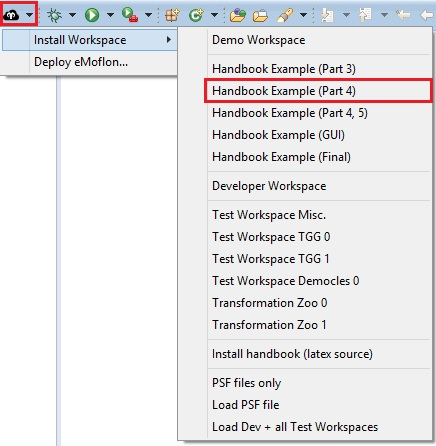
\includegraphics[width=0.65\textwidth]{eclipse_part4FreshWizardDownload}
  \caption{Initialize your workspace}
  \label{eclipse:downPartIV}
\end{center}
\end{figure} 

If you ever want to create your own meta-model, eMoflon provides a wizard (\menuPath{Create new repository project} in the eMoflon toolbar) for this, which creates the expected project structure with an empty ecore file that you can fill out.

%%% Local Variables: 
%%% mode: latex
%%% TeX-master: "../../src/TGG_mainFile"
%%% End: 
